\documentclass[12pt,usenames,dvipsnames]{article}
\usepackage{graphicx}
\usepackage{amsmath, amsthm, amssymb, tikz, enumerate, dsfont, mathabx, mathtools}
\usepackage[english]{babel}
\usepackage{tcolorbox}
\usepackage{subfigure}
\usepackage{graphicx}
\usepackage[utf8]{inputenc}
\usepackage{minted}
\usepackage{stmaryrd}
\usepackage{cancel}
\usepackage{listings}
\usepackage{mathrsfs}
\usepackage{caption}
\usepackage{enumitem}
\usepackage{enumerate}
\usepackage[version=3]{mhchem}
\usepackage{float}
\usepackage{color}
\usepackage{siunitx}
\usepackage{array}
\usepackage{longtable}
\usepackage{csquotes}
\usepackage{indentfirst}
\usepackage{subcaption}
\usepackage{subfiles}
\usepackage{url}
\usepackage{adjustbox}
\usepackage{hyperref}
\usepackage[sorting=none]{biblatex}
\usepackage{cleveref}
\bibliography{references} % Name of your .bib file (without extension)

\usepackage{xcolor}   % Needed to define custom colors
\usepackage{xltabular}
\usepackage{booktabs}
\usepackage{array}
\usepackage{ragged2e}
\usepackage{graphicx}

\usepackage{helvet}
\renewcommand{\familydefault}{\sfdefault}


% Definindo a cor cinza claro
\definecolor{lightgray}{gray}{0.9}
\definecolor{lightgray}{gray}{0.95}

% Define custom colors for the style
\definecolor{backcolour}{rgb}{0.95,0.95,0.92} % Light grey background
\definecolor{codegreen}{rgb}{0,0.6,0}         % Green for comments
\definecolor{codegray}{rgb}{0.5,0.5,0.5}      % Gray for line numbers
\definecolor{codepurple}{rgb}{0.58,0,0.82}    % Purple for strings
\definecolor{magenta}{rgb}{0.85, 0, 0.85}     % Magenta for keywords
\definecolor{darkblue}{rgb}{0.1, 0.1, 0.6}        % Dark blue for keywords
\definecolor{yellow}{rgb}{1, 1, 0.4}              % Yellow for functions
\definecolor{codeblue}{rgb}{0.5, 0.8, 1}          % Light blue for variables
\definecolor{lightgreen}{rgb}{0.6, 1, 0.6}        % Light green for numbers
\definecolor{black}{rgb}{0.1, 0.1, 0.1}      % Black color
\definecolor{darkgreen}{rgb}{0.0, 0.5, 0.0}
\definecolor{rowgray}{gray}{0.95}


% Define Python style
\lstdefinestyle{Pythonstyle}{
    language=Matlab,                % programming language
    backgroundcolor=\color{backcolour},   % background color
    commentstyle=\color{codegreen},       % comment style
    keywordstyle=\color{darkblue},         % keyword style
    numberstyle=\tiny\color{codegray},    % the style used for the line-numbers
    stringstyle=\color{codepurple},       % string literal style
    emph={np},            % highlight function names
    emphstyle=\color{darkblue},             % yellow for function names
    basicstyle=\ttfamily\footnotesize,    % the size of the fonts used for the code
    breakatwhitespace=false,              % sets if automatic breaks should only happen at whitespace
    breaklines=true,                      % sets automatic line breaking
    captionpos=b,                         % sets the caption-position to bottom
    keepspaces=true,                      % keeps spaces in text
    numbers=left,                         % where to put the line-numbers
    numbersep=5pt,                        % how far the line-numbers are from the code
    showspaces=false,                     % show spaces everywhere adding particular underscores
    showstringspaces=false,               % underline spaces within strings only
    showtabs=false,                       % show tabs within strings adding particular underscores
    tabsize=2                             % sets default tabsize to 2 spaces
}


\newcommand{\PR}[1]
{\ensuremath{\left[#1\right]}}
\newcommand{\PC}[1]
{\ensuremath{\left(#1\right)}}
\newcommand{\chav}[1]
{\ensuremath{\left\{#1\right\}}}
\allowdisplaybreaks
\DeclareMathOperator{\sen}{sen}
\DeclareMathOperator{\tg}{tg}
\DeclareMathOperator{\cotg}{cotg}
\graphicspath{{Figures/}}
\addtolength{\textwidth}{1in}
\addtolength{\textheight}{1in}
\addtolength{\evensidemargin}{0.5in}
\addtolength{\oddsidemargin}{-0.5in}
\addtolength{\topmargin}{-0.5in}

\theoremstyle{definition}
\newtheorem{definition}{Definição}[subsection]
\newtheorem{theorem}{Teorema}[subsection]
\newtheorem{example}{Exemplo}[subsection]
\newtheorem{prop}{Proposição}[subsection]
\newtheorem{lem}{Lema}[subsection]
\theoremstyle{remark}
\newtheorem*{remark}{Remark}




\begin{document}
\begin{titlepage}
	\noindent\rule{\textwidth}{1pt}
    \noindent
    \begin{minipage}[t]{0.48\textwidth}
      \textbf{LT8390}
    \end{minipage}%
    \hfill%
    \begin{minipage}[t]{0.48\textwidth}
      \raggedleft
      \textbf{Régulateur sélectionnable Buck-Boost} \\
	  \textbf{à commande opto-isolée}
    \end{minipage}\\[0.5em]

    \vspace{1cm}

    \noindent
    \begin{minipage}[t]{0.48\textwidth}
	\textbf{Description Générale}

	\vspace{0.5cm}

	Ce projet présente la conception et la réalisation d'une carte convertisseur DC-DC compacte et haute performance, basée sur le contrôleur synchrone à 4 interrupteurs LT8390 de Linear Technology. La carte accepte une large plage de tensions d'entrée (8 V-56 V) et fournit une sortie réglable de 0 V à 56 V en mode Buck-Boost ou jusqu'à Vin en mode Buck, avec contrôle de courant cycle-par-cycle jusqu'à 30 A en entrée et rendements de crête supérieurs à 93 \%.

	\vspace{0.3cm}

	Les blocs fonctionnels clés comprennent : une étage Buck-Boost intégré, une protection contre l'inversion de polarité à base de MOSFET, un convertisseur auxiliaire Fly-Buck (LM5160A) fournissant des rails 5 V isolés et non isolés, une interface de contrôle externe galvanique isolée (0-5 V ou 4-20 mA) basée sur l'optocoupleur HCNR200, et un réseau programmable de sélection de mode et d'injection de rétroaction (utilisant un PWM LTC6992 pour l'échelle Buck).

	\vspace{0.3cm}

	Le cycle complet de développement a été réalisé : définition de la topologie et dimensionnement des composants selon les datasheets, modélisation LTspice, implantation du PCB sous Altium, et validation en banc des étages de puissance et des boucles de contrôle.

	\end{minipage}%
	\hfill%
	\begin{minipage}[t]{0.48\textwidth}
	\textbf{Avantages et Caractéristiques}

	\begin{itemize}[leftmargin=0pt,labelsep=5pt]
		\item Plage de tension d'entrée étendue (8V-56V).
		\item Topologie synchrone 4 interrupteurs LT8390.
		\item Rendement $>$ 93\%.
		\item Protection contre inversion de polarité par MOSFET avec indication LED visuelle.
		\item Convertisseur auxiliaire Fly-Buck fournissant des rails 5 V isolés et non isolés.
		\item Contrôle externe galvanique isolé via optocoupleur haute linéarité.
		\item Interface de commande externe sélectionnable (0-5 V ou 4-20 mA).
		\item Sélection dynamique du mode entre Buck-Boost (0 V-56 V en sortie) et Buck (0 V-Vin en sortie).
		\item Limitation de courant cycle-par-cycle (résistance de détection 1,6 m$\Omega$), UVLO ($>$ 8 V) et démarrage progressif pour protection robuste.
		\item Modulation de fréquence à Spread Spectrum pour réduire les EMI.
		\item PCB compact 2 couches à haute densité de composants.
	\end{itemize}
	\end{minipage}


    \vfill

    \noindent
    \begin{minipage}[t]{0.48\textwidth}
      \footnotesize Révision 1 - Juin 2025 \\
    \end{minipage}%
    \hfill%
    \begin{minipage}[t]{0.48\textwidth}
      \raggedleft
    \end{minipage}\\[0.5em]

\end{titlepage}


\section{Outils Utilisés}

Pour le développement complet de ce projet, trois outils principaux ont été utilisés : LTspice, LTpowerCAD et Altium Designer. Chacun d'eux joue un rôle fondamental à différentes étapes du processus de création, depuis la simulation et le dimensionnement initial des composants jusqu'à l'élaboration des schémas et du circuit imprimé (PCB).

LTspice est un simulateur SPICE de circuits électroniques gratuit, fourni par Analog Devices. Il permet de modéliser des transistors, diodes, inductances, condensateurs et de nombreux autres composants électroniques, en réalisant des analyses dans le domaine temporel (transitoires), fréquentiel (balayage AC) et en point de fonctionnement (point DC), entre autres. Dans le cadre de ce projet, LTspice a été utilisé pour simuler tous les sous-circuits conçus. Grâce à ces simulations, il a été possible d'observer les formes d'onde de commutation, d'analyser les ondulations de tension et de courant, d'estimer les rendements et de valider les circuits de protection avant l'assemblage physique de la carte. L'outil a également facilité l'ajustement des valeurs des inductances, résistances de détection et fréquences de commutation, rendant le processus de dimensionnement plus efficace et précis. La simulation a permis d'identifier d'éventuels problèmes de stabilité et de bruit, permettant ainsi des ajustements avant la fabrication du prototype. Cependant, elle ne permet pas de valider les protections contre les interférences électromagnétiques (EMI) et la compatibilité électromagnétique (EMC), qui sont extrêmement difficiles à évaluer sans la réalisation physique du circuit.

LTpowerCAD est un logiciel d'aide à la conception de régulateurs de puissance, également proposé par Analog Devices. Cet outil automatise le dimensionnement initial des convertisseurs DC/DC, en suggérant des valeurs pour les inductances, condensateurs, MOSFETs et résistances de rétroaction en fonction des paramètres d'entrée (tension d'alimentation, tension de sortie désirée, courant de charge, fréquence de commutation, entre autres). Pour le convertisseur buck-boost principal, LTpowerCAD a été utilisé pour générer une conception de base, en définissant des valeurs approximatives d'inductance, de capacité et de composants de contrôle recommandés par le fabricant du LT8390. À partir de cette base, les paramètres ont été affinés dans LTspice, garantissant que les aspects théoriques et pratiques du projet respectaient les critères d'efficacité, de stabilité et de robustesse définis dans la fiche technique.

Enfin, Altium Designer a été l'outil choisi pour le développement du schéma complet et de la carte de circuit imprimé (PCB). Altium Designer est un environnement de conception assistée par ordinateur (CAO) dédié à l'électronique, permettant de dessiner les schémas, créer des bibliothèques de composants, définir les règles de conception (design rules) et réaliser des layouts de cartes avec des fonctions avancées de routage, d'analyse d'intégrité du signal et de vérification d'impédance. Dans le cadre de ce projet, Altium Designer a permis la capture schématique de tous les sous-circuits, la connexion des signaux d'alimentation et de commande, l'insertion de composants spécifiques (LT8390, LM5160A, optocoupleurs, MOSFETs, etc.), et ensuite la génération du PCB avec un empilement de couches approprié, la définition des vias, des plans de cuivre pour l'alimentation et des zones de masse optimisées. De plus, Altium a généré les fichiers de fabrication (Gerber, NC Drill et listes de matériaux) nécessaires à la production du prototype, assurant que le projet respecte les bonnes pratiques de routage et les exigences de fabrication industrielle.




\section{Sous-circuits}

Dans cette section, sont présentés les principaux blocs qui composent la carte : (1) le convertisseur Buck-Boost basé sur le LT8390, chargé de la conversion DC/DC de la tension d'entrée vers la tension de sortie désirée , (2) le circuit de protection contre l'inversion de polarité, qui empêche tout dommage si les câbles d'alimentation sont inversés , (3) le convertisseur Fly-Buck, qui génère les alimentations 5 V nécessaires aux circuits de commande, tant en zones isolée que non isolée , (4) le circuit de signal de commande externe isolé, qui reçoit et conditionne des signaux 0-5 V ou 4-20 mA de manière galvanisée isolée , et (5) le circuit de commande et de sélection de mode, chargé d'adapter et d'injecter le signal de commande dans la boucle de rétroaction du LT8390, permettant de choisir entre les modes Buck et Buck-Boost et d'ajuster la tension de sortie selon la valeur du signal externe. Chaque sous-circuit sera détaillé ci-après, présentant son principe de fonctionnement, le dimensionnement des composants et son intégration au système global.

\subsection{Convertisseur Buck-Boost}

Le cœur fonctionnel de la carte est constitué par le convertisseur DC-DC en topologie buck-boost, implémenté avec le contrôleur synchrone LT8390. Comme illustré à la Figure \ref{fig:lt8390}, le LT8390 intègre un contrôleur à quatre interrupteurs (MOSFETs Q2, Q3, Q4 et Q5 sur la Figure \ref{fig:buck_boost_converter}) autour d'un unique inducteur (L1), autorisant le fonctionnement en mode buck, boost ou buck-boost sans circuits externes supplémentaires pour la gestion des transitions de mode. Le dimensionnement de tous les composants (filtres, inducteurs, condensateurs de découplage et résistances de détection de courant) s'appuie sur les calculs et recommandations du datasheet du LT8390, garantissant que le circuit respecte les exigences de performance et de fiabilité du fabricant.

\begin{figure}[H]
    \centering
    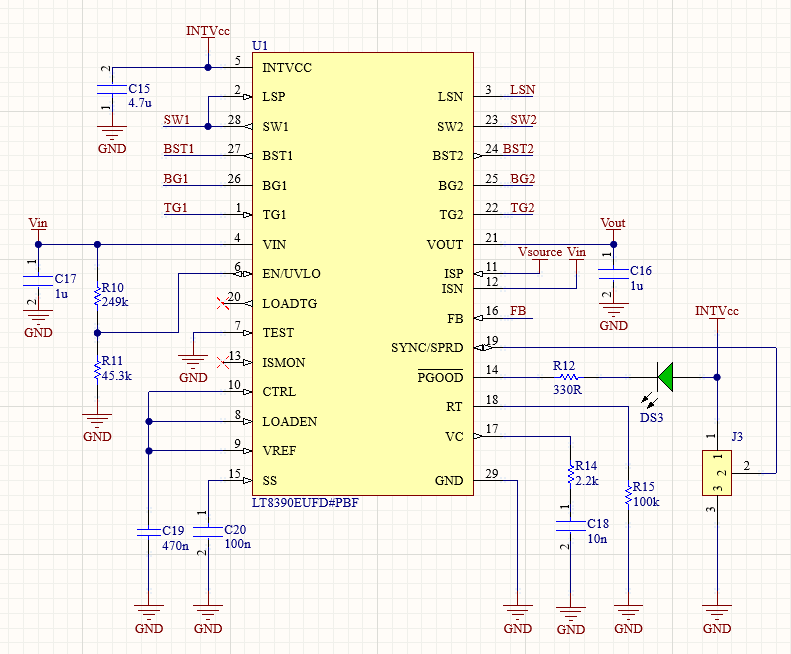
\includegraphics[width=0.9\textwidth]{figures/LT8390.png}
    \caption{Schéma du contrôleur LT8390}
    \label{fig:lt8390}
\end{figure}

\begin{figure}[H]
    \centering
    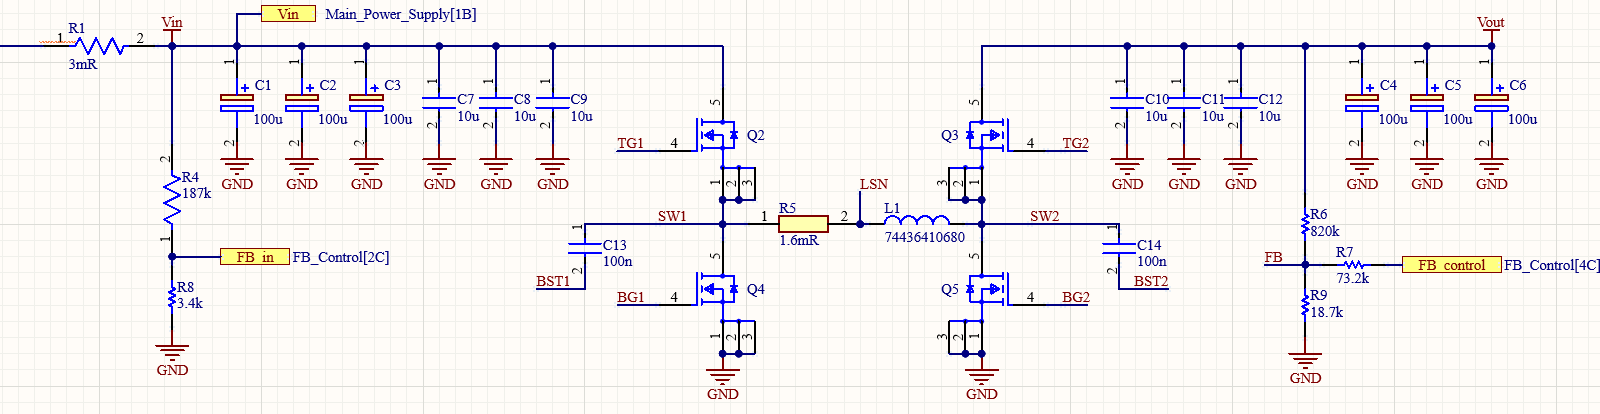
\includegraphics[width=1\textwidth]{figures/PowerStage.png}
    \caption{Topologie du convertisseur Buck-Boost synchrone à 4 interrupteurs}
    \label{fig:buck_boost_converter}
\end{figure}

Le LT8390 utilise un contrôle en crête de courant, applicable tant en abaissement qu'en élévation de tension, en mesurant le courant de l'inducteur via une résistance de détection de faible valeur (R5, 1,6 m$\Omega$, voir Figure \ref{fig:buck_boost_converter}). Cette résistance est continuellement surveillée par les entrées LPS et LSN du contrôleur, permettant une régulation cycle par cycle et une protection contre les surintensités, comme détaillé dans le datasheet. La précision du contrôle de courant, associée à la commutation synchrone à haute fréquence (400 kHz, réglée par la résistance R15), offre des rendements supérieurs à 95\% sur la majeure partie de la plage de fonctionnement, et pouvant atteindre 98\% selon l'exemple de référence du fabricant. Dans ce projet, l'efficacité maximale simulée en conditions optimales a été de 93\%, satisfaisante pour une application aux limites de tension et de courant spécifiées par le LT8390.

Pour atténuer les bruits et interférences électromagnétiques susceptibles d'induire des signaux parasites sur les pistes voisines, de déstabiliser la boucle de régulation ou d'émettre vers d'autres équipements sensibles, le LT8390 intègre une modulation de fréquence à spectre étalé (spread-spectrum). Plutôt que de toujours commuter à une fréquence fixe, dont les composantes spectrales concentrées risqueraient de violer les normes EMI ou de brouiller des circuits RF voisins, cette modulation fait fluctuer légèrement la fréquence de commutation dans le temps, répartissant l'énergie sur une bande plus large et réduisant ainsi les pics de densité spectrale. L'activation de cette fonction s'effectue via le jumper J3 (broche SYNC/SPRD) sur la Figure \ref{fig:lt8390}. Dans les applications où de faibles pics de bruit peuvent nuire à des circuits analogiques ou des modules RF (télécommunications, instruments de mesure sensibles), le spread-spectrum est particulièrement avantageux.

Le contrôleur offre en outre un soft-start (broche SS), une protection UVLO (Under Voltage Lockout) en cas de sous-tension d'entrée, ainsi qu'une protection interne contre les courts-circuits et surcharges, avec possibilité de redémarrage automatique ou de latch-off, selon le manuel technique du LT8390.

Lors de la phase de conception, un réseau de découplage et de filtrage a été mis en place, comportant plusieurs condensateurs en entrée et en sortie, essentiel pour limiter le bruit, amortir les transitoires et stabiliser la boucle de régulation. Les valeurs d'inductance et de capacité ont été calculées d'après les formules de ripple de courant et de tension du datasheet, garantissant que le courant de crête reste en dessous des limites du fabricant et que la tension de sortie demeure stable même lors de variations rapides de charge. Le ripple tensionnel pico-pico maximal projeté était de 900 mV pp, d'où l'emploi de condensateurs d'entrée (C1, C2, C3, C7, C8, C9) et de sortie (C4, C5, C6, C10, C11, C12) de 10 µF et 100 µF à faible ESR, comme recommandé par le LT8390.

En fonctionnement, le convertisseur accepte une tension d'alimentation de 8 V à 56 V en entrée (broche VIN du LT8390) et se met en veille si la tension descend en dessous de 8 V (grâce à l'UVLO interne). Le courant d'entrée maximal projeté est de 30 A, dimensionné par la résistance de détection et les MOSFETs, pour répondre à des charges lourdes. En mode buck-boost, la tension de sortie est réglable entre 0 V et 56 V, tandis qu'en mode buck strict, la sortie varie de 0 V à la tension d'entrée (Vin). La sélection du mode s'effectue via un interrupteur dédié sur le PCB, mais c'est le LT8390 qui, selon la référence de tension présente sur la broche FB (alimen­tée par la commande externe, détaillée ultérieurement), pilote la commutation des MOSFETs pour atteindre la tension désirée. Les résistances de rétroaction R6, R7 et R9 (Figure \ref{fig:buck_boost_converter}) définissent le rapport entre la tension de sortie et le signal de feedback, assurant une opération stable sur l'ensemble de la plage 0-56 V.






\subsection{Protection contre l'inversion de polarité}

La protection contre l'inversion de polarité sur cette carte est réalisée à l'aide d'un circuit à base de MOSFET, qui bloque tout courant si la source d'alimentation est connectée à l'envers, tout en maintenant des pertes très faibles. Cette configuration empêche la tension de sortie d'être inversée et protège à la fois le convertisseur et les autres blocs de la carte en cas d'inversion accidentelle des câbles sur les connecteurs d'entrée.

Comme illustré à la Figure \ref{fig:reverse_polarity_protection}, la tension d'entrée (Vsource) arrive sur le drain du MOSFET Q1 (dont le diode de corps interne est orienté pour bloquer les courants inverses) et, lorsque la source est correctement connectée, circule vers le reste du circuit avec une chute de tension négligeable grâce à la faible valeur de \(R_{DS(\text{on})}\). La gate de Q1 est référencée au drain via un pont diviseur et un diode Zener (D1), qui limite la tension \(V_{GS}\) pour ne pas dépasser la limite sûre du MOSFET. Dans cette condition de polarité correcte, la tension appliquée à la gate reste légèrement négative par rapport à la source (selon le modèle de MOSFET), forçant Q1 à rester parfaitement saturé. Simultanément, la LED verte (DS2) s'allume, indiquant « alimentation correcte », car son anode est relié à Vsource et son cathode au point COM.

\begin{figure}[H]
    \centering
    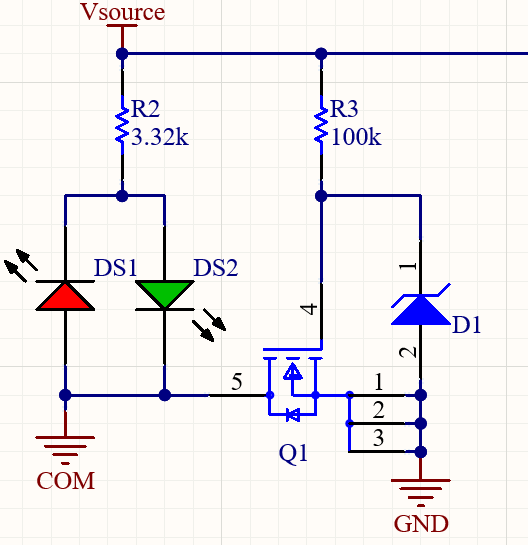
\includegraphics[width=0.5\textwidth]{figures/ReversePolarity.png}
    \caption{Circuit de protection contre l'inversion de polarité}
    \label{fig:reverse_polarity_protection}
\end{figure}

En cas d'inversion de polarité, la source négative se retrouve sur le drain de Q1, mais le diode de corps interne bloque tout passage de courant dans ce sens. De plus, la tension d'entrée inversée rend le nœud de gate plus positif que la source, ce qui fait dépasser \(V_{GS}\) du seuil de conduction et force Q1 à s'éteindre complètement. Le diode Zener D1 garantit que cette surtension sur la gate ne détériore pas le transistor, tandis que la résistance \(R_3\) (en série avec D1) limite le courant traversant le Zener, maintenant \(V_{GS}\) à un niveau sûr. Dans cette situation, la LED rouge (DS1) s'allume, car elle ne conduit que lorsque l'entrée est inversée, signalant « polarité incorrecte ».

En résumé, le point clé de ce schéma est la topologie « MOSFET inversé » : le corps de Q1 sert de diode de blocage en cas d'inversion, la gate est maintenue à une tension qui l'empêche de conduire, et la combinaison d'un pont diviseur et d'un diode Zener garantit qu'au reconnecter la source correctement, la gate est tirée légèrement sous la source, autorisant une conduction normale avec une chute de tension minimale. En d'autres termes, en connexion correcte, le MOSFET conduit sans pertes significatives , en connexion inversée, il reste fermé, protégeant le convertisseur et les circuits en aval. Les LEDs offrent une indication visuelle immédiate de l'état de la connexion.

Ainsi, le circuit de protection contre l'inversion de polarité utilise un unique MOSFET à diode de corps interne, une résistance de gate et un diode Zener pour limiter \(V_{GS}\). Grâce à cette combinaison, le schéma assure une protection instantanée en cas d'inversion des câbles, présente des pertes de conduction quasi nulles en configuration correcte et indique visuellement le statut de la connexion via des LEDs dédiées.


\subsection{Sources d'Alimentation Internes de 5V (Convertisseur Fly-Buck)}

La carte nécessite plusieurs sources d'alimentation basse tension pour ses composants de commande, ses tensions de référence et ses circuits intégrés (CI), couvrant à la fois la partie isolée et la partie non isolée du système. Pour répondre à ce besoin, qui consiste à convertir la haute tension d'entrée principale du circuit (comprise entre 8 V et 56 V, comme spécifié par le projet) en niveaux de 5 V, un convertisseur DC/DC en topologie Fly-Buck a été implémenté. Ce choix est stratégique, car il permet de générer des sorties isolées, ce qui est idéal pour alimenter des circuits ne devant pas être en contact direct avec le bus principal, comme le circuit de signal de commande isolé. Le cœur de cette solution est le contrôleur LM5160A de Texas Instruments, un CI robuste et efficace conçu à cet effet.

Comme illustré à la Figure \ref{fig:flybuck_schematic}, ce circuit constitue la source principale alimentant tous les circuits isolés et non isolés de la carte. Il utilise une topologie développée par Texas Instruments qui combine les caractéristiques d'un convertisseur Buck, capable d'abaisser une tension d'entrée pour en obtenir une autre, et d'un convertisseur Flyback, où une tension de sortie isolée est générée à partir de l'entrée. Cet agencement est employé pour réduire la tension d'entrée, qui peut atteindre 56 V, en deux sources d'alimentation basse tension : une non isolée, destinée à alimenter tous les composants (CI, amplificateurs opérationnels, génération de signaux de référence), et une isolée, dédiée à l'alimentation du circuit de signal de commande isolé. Cette topologie constitue une solution très efficace, capable de fournir toutes les sources nécessaires pour l'ensemble des sous-systèmes de la PCB. De plus, elle offre une haute efficacité et une faible dissipation de puissance, minimisant l'impact sur l'efficacité globale du convertisseur Buck-Boost principal.

\begin{figure}[H]
\centering
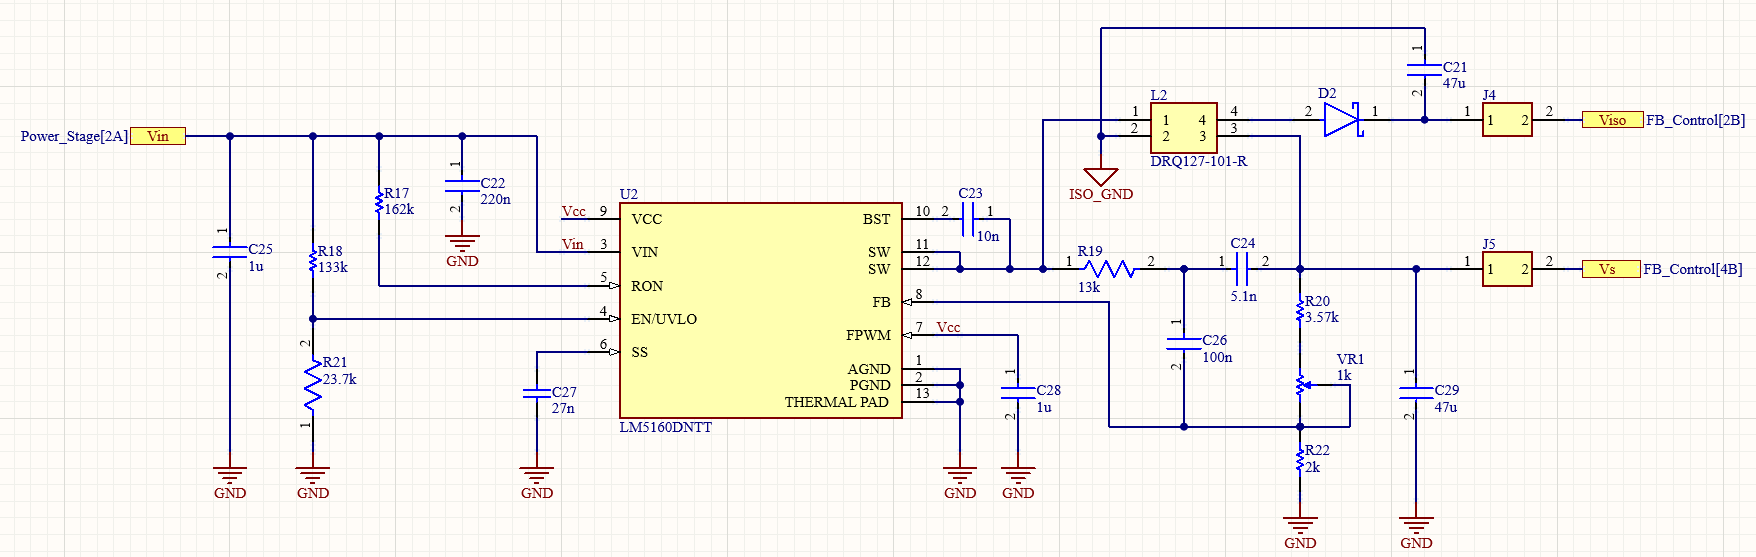
\includegraphics[width=0.9\textwidth]{figures/PowerSupply.png}
\caption{Schéma du Convertisseur Fly-Buck}
\label{fig:flybuck_schematic}
\end{figure}

Le circuit d'alimentation interne de 5 V est centré sur le contrôleur LM5160A de Texas Instruments (U2 dans le schéma), un convertisseur abaisseur synchrone (step-down) 65 V/2 A qui se distingue par l'intégration de MOSFETs haute et basse latéral. Cette intégration supprime le besoin de diodes Schottky externes pour la rectification, contribuant directement à l'efficacité en réduisant les pertes de conduction et simplifiant la nomenclature (BOM) ainsi que le routage de la carte. Le LM5160A fonctionne selon un schéma de contrôle en temps de conduction constant adaptatif (COT), qui dispense de toute compensation de boucle externe, simplifiant le design et offrant une réponse transitoire rapide. La fréquence de commutation, réglable par un simple résistor, peut atteindre 1 MHz et reste pratiquement constante.

La capacité du LM5160A à opérer en mode PWM forcé (FPWM) est essentielle pour son usage en topologie Fly-Buck à sorties multiples, garantissant un transfert d'énergie régulier vers les sorties isolées même en cas de faible charge. Le CI intègre également des protections robustes, telles que la limitation de courant de pic, la protection UVLO (Under Voltage Lockout) et le déclenchement thermique, renforçant la fiabilité. La nature synchrone du LM5160A, utilisant des MOSFETs plutôt que des diodes en basse latéral, est cruciale pour l'opération Fly-Buck, car une diode bloquerait le courant inversé nécessaire pour transférer l'énergie vers la sortie isolée.

La topologie Fly-Buck est une variante du convertisseur Buck synchrone, où l'inducteur traditionnel est remplacé par un inducteur couplé (L2 dans le schéma) possédant plusieurs enroulements. Cette modification permet au circuit non seulement de générer une sortie non isolée, comme un Buck conventionnel (Vs), mais aussi de produire une ou plusieurs sorties isolées (Viso), de manière analogue à un Flyback.

La sortie non isolée est générée côté primaire de l'inducteur couplé et est directement régulée par la boucle fermée du LM5160A. Sa tension est déterminée par le rapport cyclique \(D\) et la tension d'entrée \(V_{\text{in}}\), selon la relation \(V_{\text{out1}} = D \times V_{\text{in}}\). Cette sortie alimente les composants de commande généraux sur la partie non isolée de la carte, le réseau de rétroaction étant composé de R19, R20, VR1 et R22. La sortie isolée provient d'un enroulement secondaire de l'inducteur couplé. La tension de cette sortie est régulée par « cross-regulation » via le couplage des enroulements, selon l'expression approximative \(V_{\text{out2}} = V_{\text{out1}} \times (N_2/N_1) - V_f\), où \(N_1\) et \(N_2\) sont les nombres de spires et \(V_f\) la chute de tension du diode secondaire (D2). Cette sortie est indispensable pour les circuits requérant un isolement galvanique.

En termes résumés, l'opération du convertisseur Fly-Buck se divise en deux phases principales, contrôlées par la commutation des MOSFETs internes du LM5160A. En mode \(T_{\text{on}}\) (High-Side activé), la tension d'entrée s'applique à l'enroulement primaire de l'inducteur couplé, emmagasinant de l'énergie, tandis que le diode D2 en sortie isolée est bloqué et le condensateur C21 alimente la charge isolée. En mode \(T_{\text{off}}\) (Low-Side activé, High-Side désactivé), la tension du primaire devient négative, polarisant D2 en direct et transférant l'énergie stockée vers la sortie isolée. Le fonctionnement en FPWM garantit que le MOSFET basse latéral reste conducteur, autorisant le courant inversé nécessaire au transfert d'énergie.

En somme, le circuit d'alimentation interne de 5 V, basé sur la topologie Fly-Buck et le contrôleur LM5160A, constitue une solution très efficace et robuste pour les besoins énergétiques de la carte. Sa capacité à générer simultanément des sorties isolées et non isolées à partir d'une seule entrée haute tension, associée à une conception simplifiée (sans optocoupleurs), une efficacité élevée et d'excellentes performances EMC, le rend idéal pour des applications industrielles exigeantes. Cet agencement assure non seulement une alimentation stable et fiable de tous les sous-systèmes, mais contribue également à l'efficacité globale et à la protection des circuits en aval, garantissant l'intégrité et le bon fonctionnement du système.






\subsection{Circuit de Signal de Commande Externe Isolé}

Le circuit isolé de la carte est chargé de recevoir un signal de commande externe, qui peut être soit au format tension (0 V à 5 V), soit au format courant (4 mA à 20 mA), et de le préparer pour le circuit principal du convertisseur Buck-Boost. Une caractéristique essentielle de ce circuit est l'isolation galvanique complète par rapport au reste de la carte, garantissant l'intégrité et la sécurité du système principal face aux bruits et transitoires de la source externe. Pour cela, le circuit intègre un sélecteur d'entrée et un amplificateur isolé analogique de haute linéarité, centré sur l'optocoupleur HCNR200. Comme illustré à la Figure \ref{fig:iso_input_control}, le circuit se divise en deux zones distinctes : la zone isolée (à gauche de la ligne pointillée rouge) et la zone non isolée (à droite), la transition étant assurée par le HCNR200 pour garantir l'isolation requise.

\begin{figure}[H]
\centering
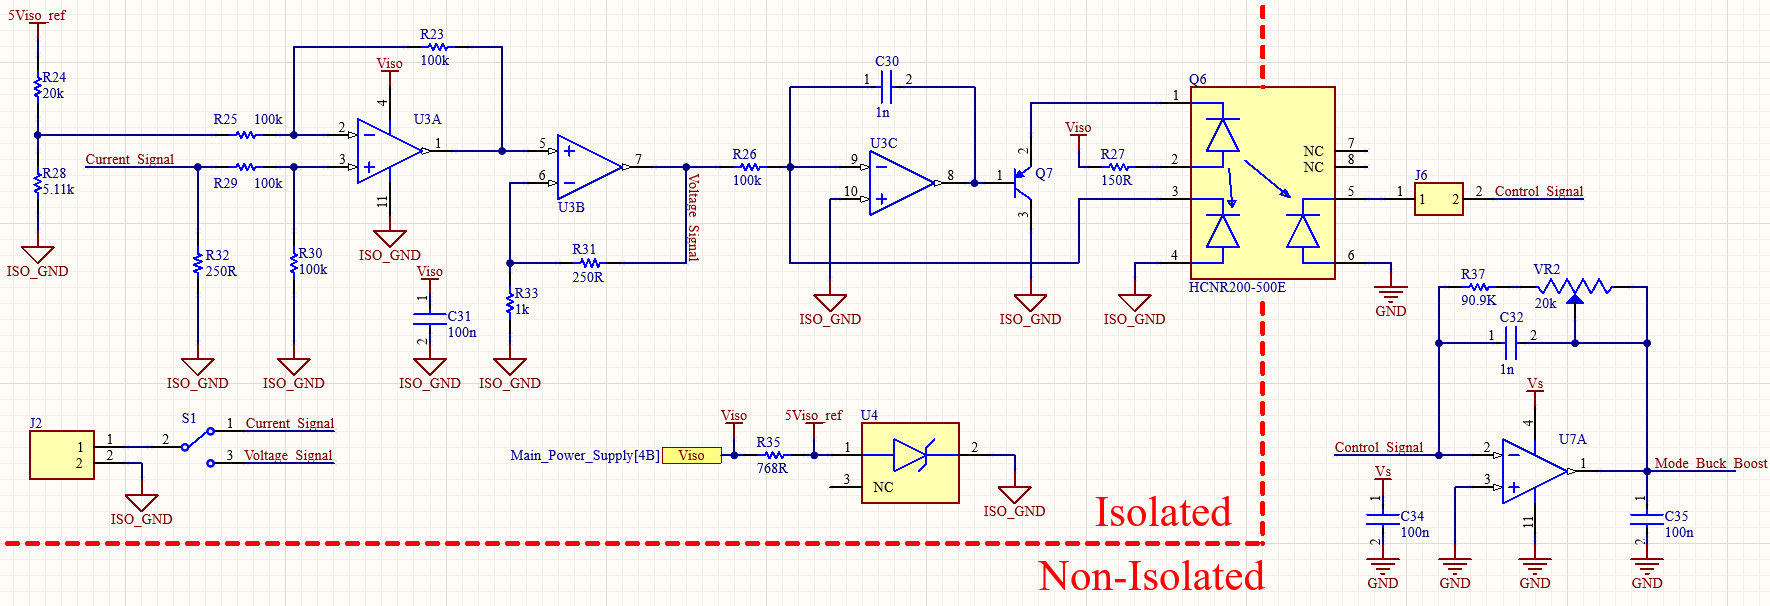
\includegraphics[width=0.9\textwidth]{IsoInputControl.png}
\caption{Circuit de signal de commande externe isolé}
\label{fig:iso_input_control}
\end{figure}

Le circuit offre à l'utilisateur la flexibilité de choisir le type de signal de commande, tension ou courant, via l'interrupteur S1. En mode tension, le signal d'entrée analogique (Voltage\_Signal) est directement dirigé vers le circuit d'isolation et transféré de la zone isolée vers la zone non isolée. En mode courant, le signal d'entrée (Current\_Signal) subit d'abord un conditionnement avant isolation. Cette étape est cruciale pour convertir le courant en une tension 0 V-5 V compatible avec le traitement suivant.

Lorsque S1 est en mode courant, le signal Current\_Signal passe par trois étapes de conversion : d'abord, une résistance de shunt de 250 $\Omega$ transforme le courant 4-20 mA en une tension de 1 V-5 V , ensuite, un amplificateur opérationnel (U3A), configuré en soustracteur, retire l'offset de 1 V du signal. Pour cela, une tension de référence de 1 V est générée à partir de la référence 5Viso\_ref produite par U4, au moyen du pont diviseur R24/R28. Cette 1 V est soustraite de la plage 1-5 V, donnant 0 V-4 V. Enfin, un second amplificateur opérationnel (U3B), avec un gain de 1,25, étend la plage 0 V-4 V à 0 V-5 V. Le signal standardisé 0-5 V est alors acheminé vers l'amplificateur isolé analogique.

L'isolation galvanique, point central du circuit, est réalisée par l'optocoupleur à haute linéarité HCNR200-500E (Q6). Ce composant robuste permet d'isoler les signaux analogiques tout en offrant stabilité, linéarité et bande passante élevées. Le HCNR200 comprend une LED haute performance qui éclaire deux photodiodes appariées (PD1 et PD2). Le processus d'isolation et de linéarisation fonctionne ainsi : le signal de tension (Voltage\_Signal), issu du mode tension ou du conditionnement en mode courant, est appliqué à l'amplificateur U3C. Cet amplificateur, assisté par le transistor Q7, contrôle le courant du LED interne du HCNR200 (broches 1-2). Une photodiode (PD1, broches 3-4) est utilisée en boucle de rétroaction avec U3C. En surveillant la lumière émise et en ajustant le courant, les non-linéarités et dérives du LED sont quasiment annulées, assurant une relation linéaire entre le signal d'entrée et l'intensité lumineuse, quel que soit la température ou l'âge du LED. La seconde photodiode (PD2, broches 5-6), optiquement couplée, génère une photocourant linéairement proportionnelle à l'intensité lumineuse. Cette photocourant est ensuite reconvertie en tension sur le côté non isolé, produisant le signal de commande final (Control\_Signal) pour le convertisseur Buck-Boost. Le parfait appariement des photodiodes et le design du boîtier garantissent la haute linéarité et la stabilité du gain. Le HCNR200 offre une isolation de 5000 Vrms, essentielle pour les applications nécessitant une sécurité élevée et une protection contre les transitoires mode commun et les boucles de masse.






\subsection{Circuit de Contrôle et Sélection de Mode}

Ce circuit final est le maillon crucial entre le signal de commande externe isolé et le contrôleur principal du convertisseur Buck-Boost, le LT8390. Sa fonction première est de recevoir le signal de commande déjà isolé, de gérer la sélection entre les modes d'opération Buck et Buck-Boost, puis d'inverser le signal de commande avant de l'envoyer à la broche de rétroaction (FB) du LT8390.

Traditionnellement, la boucle de rétroaction d'un convertisseur DC/DC est composée d'un diviseur résistif qui échantillonne la tension de sortie et la compare à une référence interne du contrôleur, ce qui définit une tension de sortie fixe. Cependant, pour des applications requérant une tension de sortie variable et ajustable dynamiquement, comme dans ce projet, une approche plus sophistiquée est nécessaire. La technique, largement utilisée dans les modules de puissance, consiste à injecter ou drainer un faible courant dans le réseau de rétroaction du régulateur. Cette injection modifie le gain effectif du diviseur, agissant comme une « résistance virtuelle » qui déplace le point de réglage du convertisseur. Plus précisément, si un courant positif est injecté au nœud de rétroaction, la tension de sortie baisse. Inversement, si un courant est prélevé (c'est-à-dire un courant négatif injecté), la tension de sortie augmente. Cette méthode offre un contrôle plus précis et flexible comparé à la simple commutation de résistances. Pour implémenter cette fonctionnalité, une troisième résistance est raccordée au nœud central du diviseur de rétroaction du LT8390, permettant l'injection du signal de commande externe en ce point. Le circuit illustré à la Figure \ref{fig:control_signal_circuit} génère ce signal de commande, qui est injecté sur la broche FB du LT8390 via cette troisième résistance, comme montré à la Figure \ref{fig:buck_boost_converter}.

\begin{figure}[H]
\centering
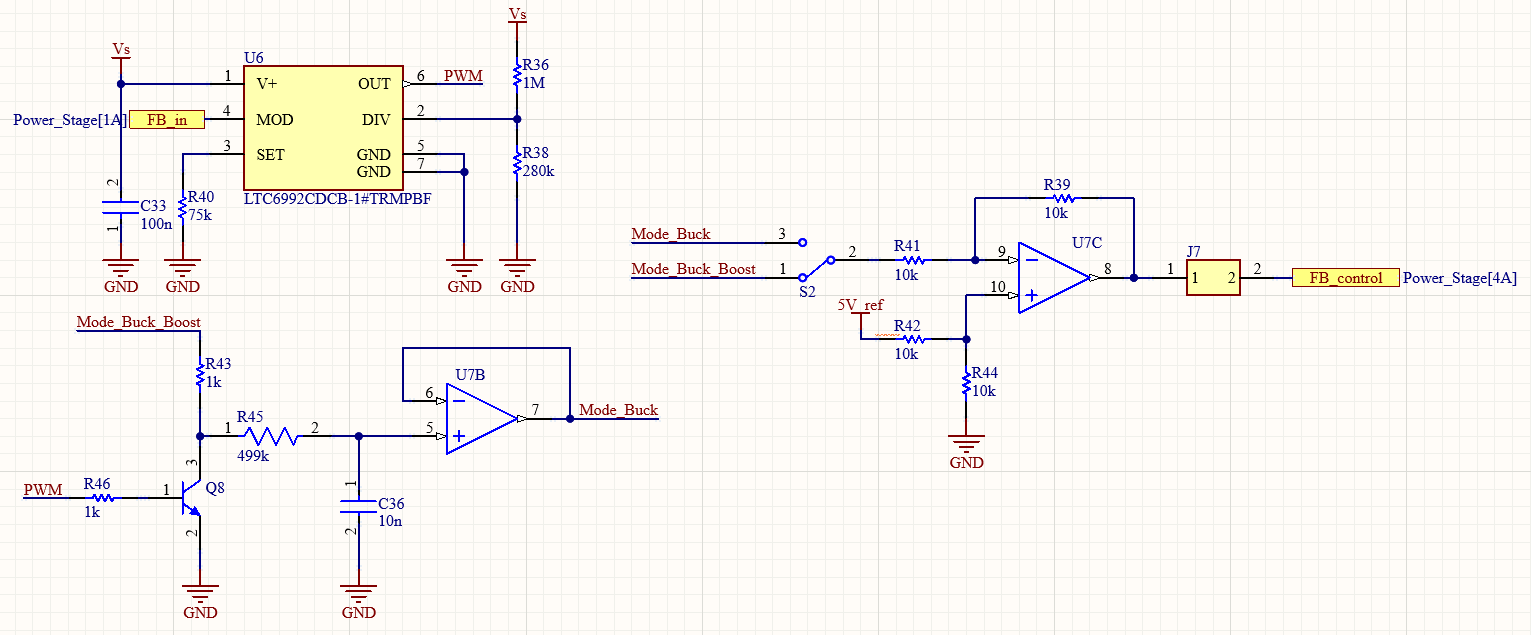
\includegraphics[width=0.9\textwidth]{ControlSignal.png}
\caption{Circuit de Contrôle et Sélection de Mode}
\label{fig:control_signal_circuit}
\end{figure}

Le circuit intègre un sélecteur de mode S2 permettant à l'utilisateur de choisir entre deux opérations distinctes : le mode Buck-Boost et le mode Buck. En mode Buck-Boost, l'objectif est que la tension de sortie du convertisseur principal varie de 0 V à 56 V en réponse à un signal de commande externe variant de 0 V à 5 V (ou 4 mA à 20 mA après conditionnement). Par exemple, un signal de commande de 0 V doit donner 0 V en sortie, tandis que 5 V en signal de commande doit conduire à 56 V en sortie. Pour obtenir cette relation, le signal de commande externe est d'abord inversé de 0-5 V en 5-0 V grâce à l'amplificateur opérationnel U7C configuré en soustracteur. L'une des entrées du soustracteur reçoit le signal de commande et l'autre une tension de référence de 5 V : lorsqu'il y a 0 V en commande, la sortie du soustracteur est 5 V (5 V - 0 V = 5 V), et lorsqu'il y a 5 V en commande, la sortie est 0 V (5 V - 5 V = 0 V).

La logique derrière cette inversion est que, pour l'injection de courant dans la boucle FB du LT8390, une tension d'injection plus élevée en FB entraîne une tension de sortie plus faible. Ainsi, un signal externe de 0 V (devenu 5 V après inversion) « tire » la FB vers le bas, diminuant la sortie à 0 V , inversement, un signal externe de 5 V (devenu 0 V après inversion) autorise la montée de la tension de sortie jusqu'à 56 V, établissant la relation inverse nécessaire. Ce signal inversé est ensuite connecté à la troisième résistance de la boucle FB du LT8390.

En mode Buck-Boost, la tension de sortie varie de 0-56 V en fonction du signal externe 0-5 V (ou 4-20 mA après conditionnement). Par exemple, 0 V commande 0 V à la sortie, 2,5 V commande 28 V, 5 V commande 56 V. Pour fonctionner dans ce mode, le signal issu du circuit de commande isolé est dirigé vers l'entrée de S2, puis passe par le circuit inverseur décrit précédemment avant d'être injecté en FB via la résistance virtuelle.

En mode Buck, la tension de sortie doit varier de 0 V jusqu'à la tension d'entrée (Vin), et non jusqu'à 56 V. Par exemple, pour Vin = 24 V, 0 V commande 0 V à la sortie sortie, 5 V commande 24 V sortie. Pour adapter le LT8390, configuré pour 56 V en Buck-Boost, à cette nouvelle plage, un circuit de contrôle transforme le signal externe en une tension de rétroaction équivalente à Vin. Cela se fait en modulant le signal externe par un PWM dont le rapport cyclique dépend de Vin. L'oscillateur LTC6992 (U6) génère ce PWM : sa broche MOD reçoit une tension FB\_in proportionnelle à Vin, modulant le duty-cycle. La sortie PWM commande Q8, puis un filtre passe-bas RC (R45, C36) convertit le PWM en tension analogique moyenne. Ce signal est enfin bufferisé par U7B, garantissant l'intégrité et l'isolation d'impédance, puis envoyé à l'autre entrée de S2. Quel que soit le mode, le signal final est ensuite inversé par U7C avant d'être relié à la broche FB du LT8390.

En somme, ce circuit est essentiel à la polyvalence et au contrôle précis de la carte. Il permet non seulement la sélection flexible entre les modes Buck et Buck-Boost, mais aussi le conditionnement et l'inversion appropriés du signal isolé pour interagir efficacement avec la boucle FB modifiée du LT8390. La combinaison de la modulation PWM pilotée par Vin et de l'injection de courant contrôlée dans FB offre un ajustement linéaire et prévisible de la tension de sortie, optimisant les performances du convertisseur principal dans diverses conditions d'exploitation.





\section{Conception de la PCB dans Altium}

Le projet de la carte de circuit imprimé (PCB) a été entièrement réalisé dans l'environnement Altium Designer, en respectant des critères techniques de performance, de fiabilité et, surtout, de coût de fabrication. Avec des dimensions finales de 100 mm sur 60 mm, la PCB a été conçue pour être aussi compacte que possible, répondant aux exigences électriques du système sans compromettre son organisation physique. Cette taille réduite, en plus de faciliter l'intégration dans des boîtiers plus petits, réduit significativement les coûts de production, notamment grâce à l'utilisation d'un simple empilement deux couches (Top et Bottom) plutôt qu'à un layout multicouche plus coûteux et complexe.

Le routage a été planifié selon les bonnes pratiques pour convertisseurs DC/DC recommandées dans le datasheet du LT8390. Des directives spécifiques ont été suivies pour le placement des MOSFETs de puissance, des condensateurs d'entrée et de sortie, des résistances de détection de courant et des autres éléments critiques. Les MOSFETs ont été positionnés au plus près de l'inducteur principal, minimisant ainsi la surface de la boucle de courant HF. Les condensateurs d'entrée sont groupés et placés à proximité de la broche VIN du LT8390 et de l'entrée du circuit, garantissant une faible inductance de piste et une réponse rapide aux transitoires. De même, les condensateurs de sortie sont situés près du nœud VOUT, assurant une faible impédance de sortie à haute fréquence. Toutes les résistances de mesure, comme R5, sont câblées en Kelvin près des broches LSP/LSN du contrôleur afin de préserver la précision de la mesure de courant et d'éviter les perturbations dans la boucle de régulation.

La couche Top regroupe tous les composants actifs et passifs, incluant les éléments de puissance, de commande et de traitement du signal. Les pistes de forte intensité sont dimensionnées en polygones larges pour supporter jusqu'à 30 A de courant d'entrée sans pertes excessives. La couche Bottom sert principalement de plan de masse continu, offrant une faible impédance de retour pour les signaux et améliorant la dissipation thermique. Les interconnexions entre Top et Bottom sont renforcées par de multiples vias, favorisant la dissipation de chaleur et maintenant l'intégrité électrique.

Chaque sous-circuit est disposé en zones bien délimitées et compactes sur la carte, avec un espacement adapté entre les blocs de puissance, de commande et de signal, ce qui facilite l'identification visuelle et la mise au point matérielle lors des tests. Les circuits sont organisés pour éviter les interférences entre signaux sensibles et pistes de commutation haute fréquence, en séparant soigneusement les plans de masse analogique et de puissance. La PCB comporte également une zone galvanique isolée, située dans le coin opposé aux connecteurs d'entrée et de sortie de tension, délimitée visuellement par un polygone de lignes blanches en sérigraphie. Cette zone abrite les circuits de signal de commande isolé, garantissant la sécurité et l'immunité aux bruits provenant de l'entrée externe. Toutes les pistes traversant cette frontière passent exclusivement par l'opto­coupleur HCNR200, assurant l'isolation électrique totale entre les parties du système.

La réalisation de la PCB utilise majoritairement des composants CMS (Component Mount Surface), ce qui permet un layout plus compact et réduit les inductances parasites sur les pistes de signal. Quelques composants THT (Through-Hole) sont toutefois présents, tels que les connecteurs, les jumpers de configuration, les interrupteurs et certains condensateurs, tous placés de manière accessible pour faciliter l'usage de sondes lors des tests en banc. L'emploi de la technologie CMS contribue également à réduire les coûts d'assemblage et à optimiser l'utilisation de l'espace disponible sur la carte.

Pour simplifier la vérification et la caractérisation du système, des jumpers et connecteurs dédiés ont été ajoutés, permettant d'activer ou de désactiver des blocs spécifiques de la carte sans intervention matérielle directe. Ces jumpers permettent, par exemple, de mettre temporairement hors service le convertisseur Fly-Buck, le circuit de protection contre l'inversion de polarité ou l'isolation de signal, facilitant ainsi les tests individuels de chaque sous-système.

Les Figures~\ref{fig:pcb_top}, \ref{fig:pcb_bottom} et \ref{fig:pcb_3d} ci-après illustrent respectivement la vue de la couche supérieure de la carte, la couche inférieure avec le plan de masse et la vue 3D complète de la PCB, mettant en évidence le positionnement des blocs principaux et l'organisation générale du projet, tandis que la Figure~\ref{fig:pcb_real} montre la carte réelle assemblée, soulignant la qualité de fabrication et la disposition des composants.

\begin{figure}[H]
    \centering
    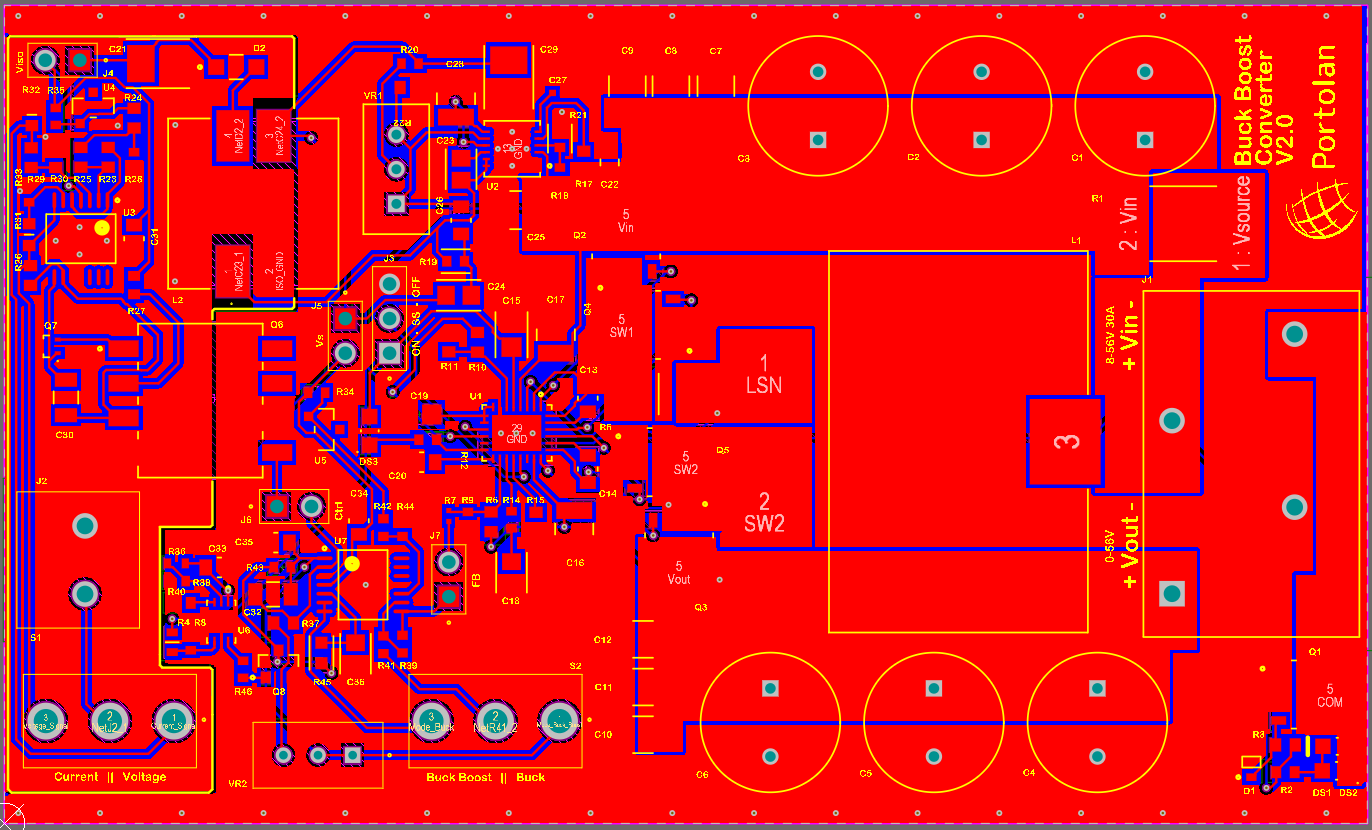
\includegraphics[width=0.8\textwidth]{figures/PCB_Top.png}
    \caption{Vue de la couche Top de la PCB avec les composants de puissance et de commande.}
    \label{fig:pcb_top}
\end{figure}

\begin{figure}[H]
    \centering
    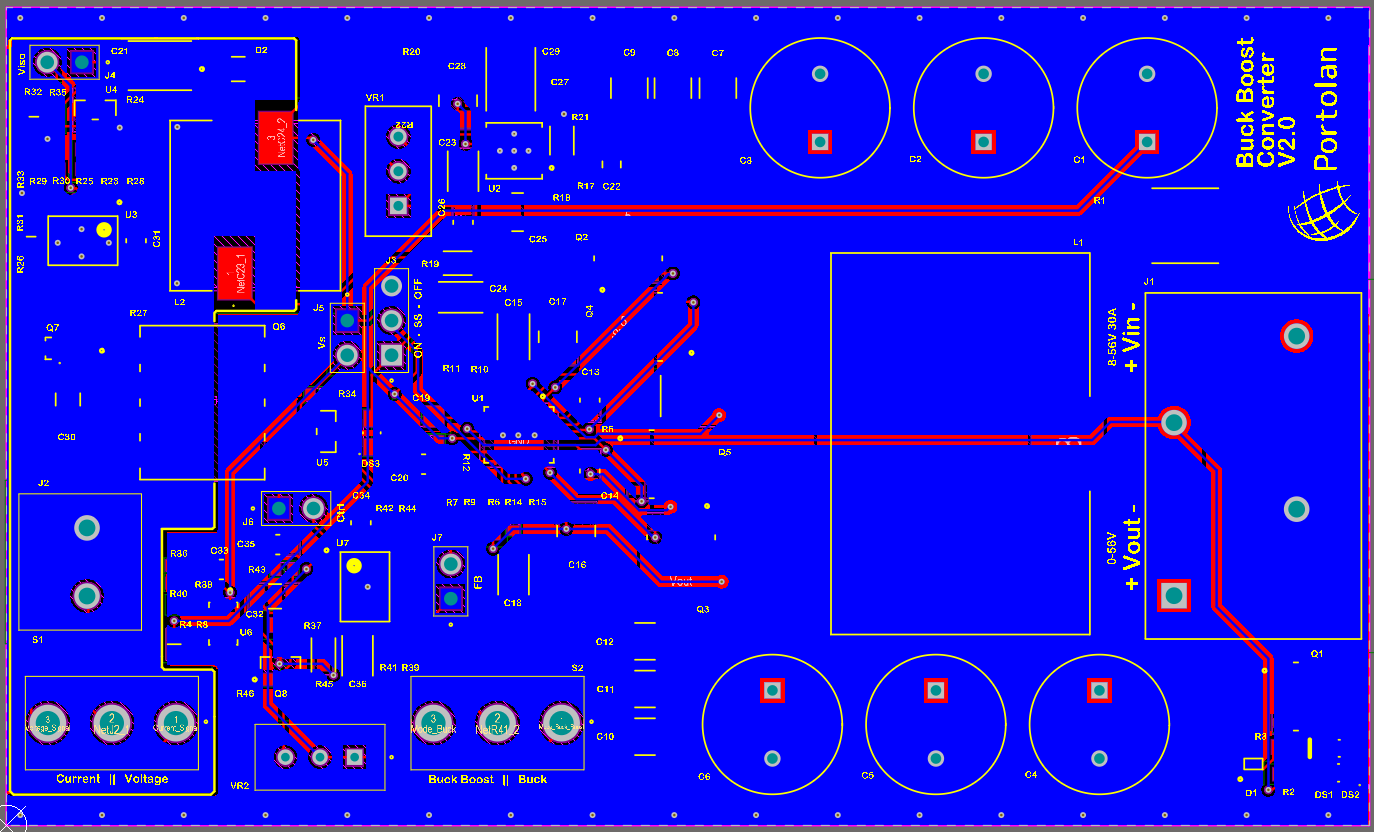
\includegraphics[width=0.8\textwidth]{figures/PCB_Bottom.png}
    \caption{Vue de la couche Bottom de la PCB, mettant en avant le plan de masse.}
    \label{fig:pcb_bottom}
\end{figure}

\begin{figure}[H]
    \centering
    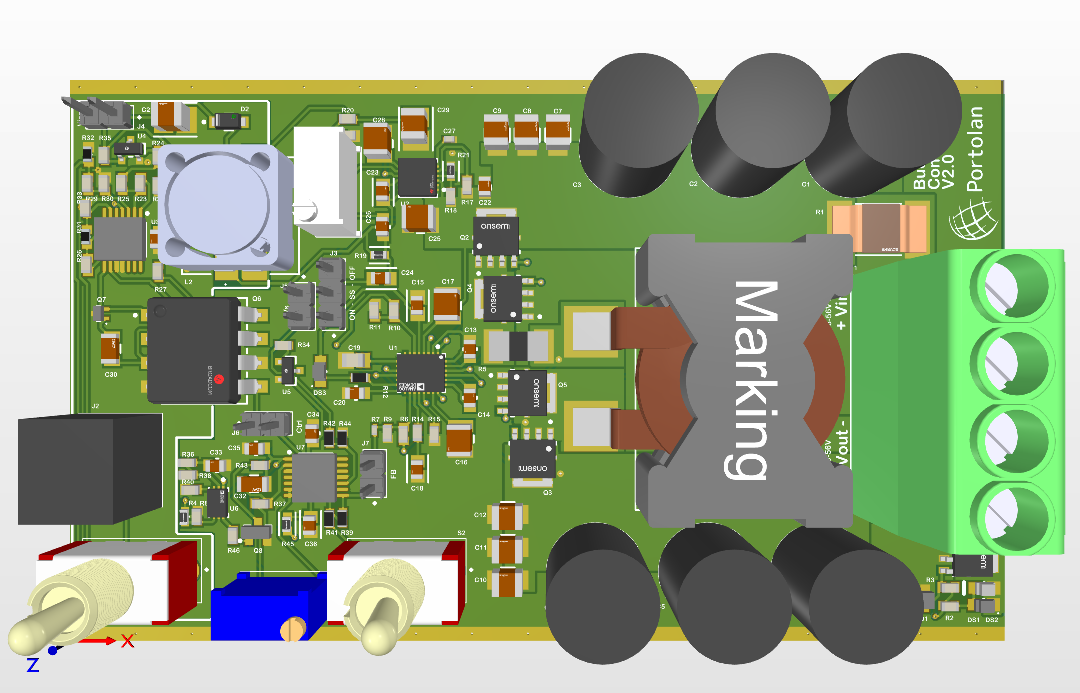
\includegraphics[width=0.8\textwidth]{figures/PCB_3D.png}
    \caption{Vue 3D du projet complet de la carte sous Altium Designer.}
    \label{fig:pcb_3d}
\end{figure}

\begin{figure}[H]
    \centering
    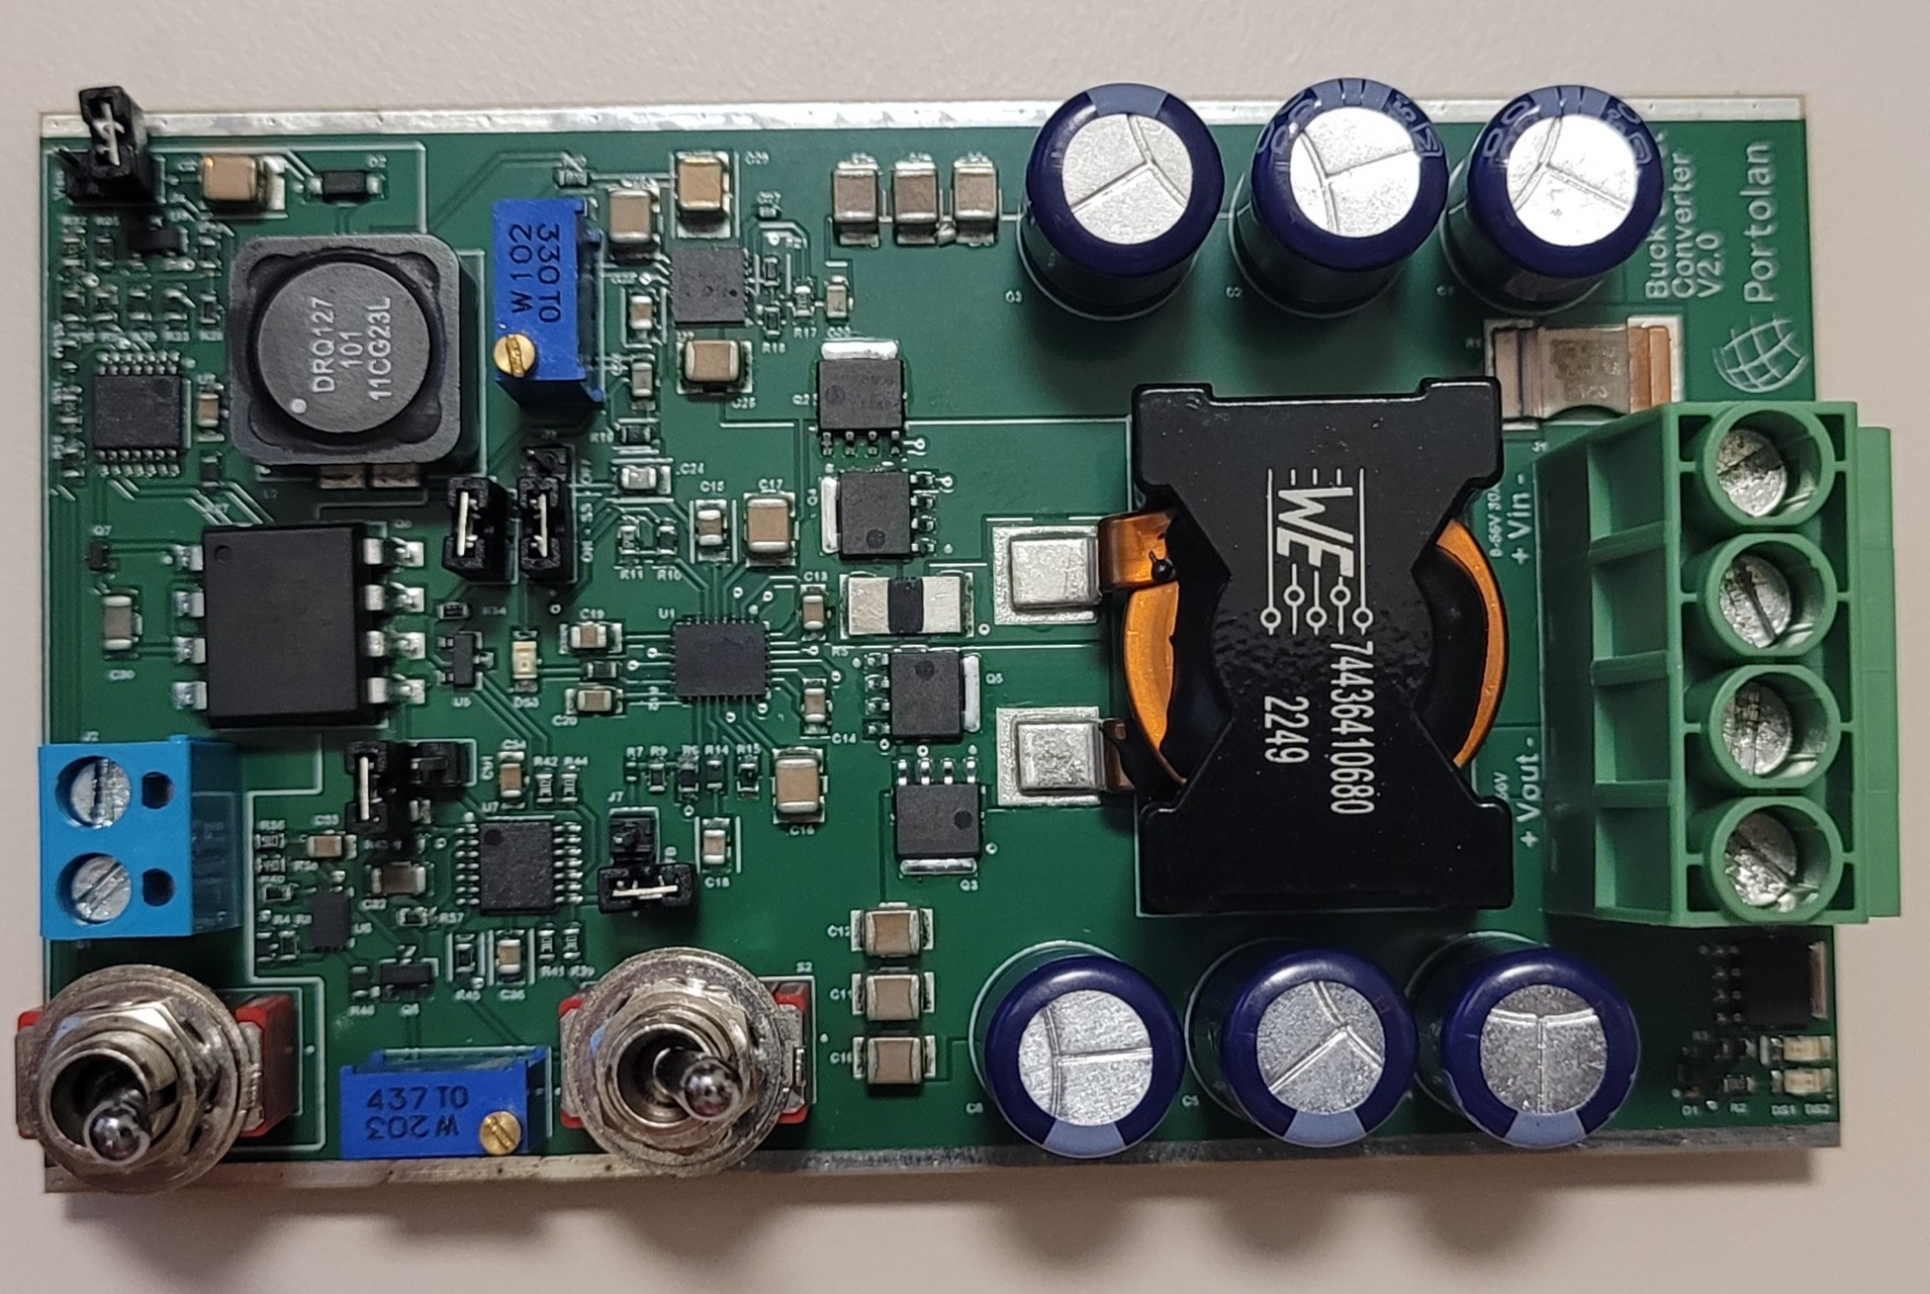
\includegraphics[width=0.8\textwidth]{figures/PCB_Real.jpg}
    \caption{Vue de la carte réelle assemblée.}
    \label{fig:pcb_real}
\end{figure}




\section{Étape de Tests}

Cette section décrit la procédure de tests effectués sur la carte développée, détaillant chaque phase de vérification, les équipements utilisés et les résultats observés lors de l'analyse fonctionnelle des sous-circuits. L'objectif était de garantir le bon fonctionnement de chaque module individuellement, ainsi que d'évaluer les performances globales de la carte en conditions réelles d'utilisation, d'identifier d'éventuelles défaillances et de valider le comportement des blocs critiques du système.

Pour la réalisation des tests, les équipements de laboratoire suivants ont été employés : un multimètre numérique pour les mesures de tension, de courant et de continuité , une pince ampèremétrique pour l'analyse de la consommation en temps réel , une alimentation variable jusqu'à 56 V pour alimenter le circuit principal , une alimentation secondaire de 5 V pour les tests isolés , un oscilloscope pour l'analyse des signaux de commande, des commutations et des bruits , ainsi que des jumpers et câbles de connexion.

Le processus de tests a débuté par une inspection visuelle minutieuse de la carte montée, afin de vérifier d'éventuelles erreurs de fabrication ou d'assemblage. Les dimensions de la PCB (100 mm x 60 mm), la présence de tous les composants prévus, leur positionnement correct, la polarité des dispositifs sensibles (condensateurs électrolytiques, diodes) et la cohérence entre le schéma Altium et la disposition physique ont été vérifiés. Le circuit a également été comparé au plan original de conception pour s'assurer qu'aucun écart structurel n'avait été introduit.

Une fois cette étape terminée, les mesures initiales ont été effectuées, notamment des tests de continuité entre les bornes d'alimentation (Vin et GND) et entre l'entrée et la sortie des blocs principaux. L'objectif était de détecter d'éventuels courts-circuits ou défauts de soudure compromettant l'alimentation. La continuité des LED a aussi été vérifiée pour contrôler le bon fonctionnement des indicateurs visuels, tant en polarité directe qu'inverse.

Avant les tests fonctionnels complets, tous les jumpers d'interconnexion entre les modules ont été retirés, permettant de tester chaque bloc de manière isolée et contrôlée. L'analyse fonctionnelle a commencé par le convertisseur Fly-Buck générant les sources internes de 5 V. Ce circuit s'est comporté comme prévu, fournissant des tensions stables aux circuits isolés et non isolés. La tension a été ajustée via le potentiomètre de calibration et est restée dans la plage spécifiée, même en charge variable.

Le circuit de protection contre l'inversion de polarité a également parfaitement fonctionné. En polarité correcte, il laissait passer la tension vers le reste de la carte et allumait la LED verte, indiquant «polarité correcte». Lors d'une inversion volontaire, il bloquait le courant et allumait la LED rouge, signalant la condition d'erreur, conformément au design théorique.

Cependant, tous les modules n'ont pas été exempts d'anomalies. Dans la zone isolée, le circuit de conditionnement et d'amplification du signal de commande a présenté de l'instabilité lors de tests prolongés. Un échauffement anormal d'un des amplificateurs opérationnels a été observé, probablement dû à un transitoire ou à une mauvaise manipulation durant les tests. Bien que le composant n'ait pas grillé, le circuit suivant de sélection de mode en a été impacté, ses entrées dépendant directement de l'étage précédent. En conséquence, les signaux injectés dans la boucle de rétroaction du LT8390 ne correspondaient pas aux valeurs attendues, compromettant le contrôle de la tension de sortie.

Concernant le convertisseur principal Buck-Boost basé sur le LT8390, toutes les tensions d'entrée étaient présentes : l'alimentation 8 V-56 V, le signal EN/UVLO, le soft-start (SS) et la référence de feedback. Pourtant, aucune tension significative n'a été générée en sortie, et la consommation restait faible et constante, sans échauffement du contrôleur, indiquant qu'il n'était ni endommagé ni en court-circuit.

Une explication possible de ce comportement inattendu est l'interférence électromagnétique générée par la commutation haute fréquence des MOSFETs et le couplage parasite dans les nœuds sensibles du circuit de commande. Cette EMI peut perturber la boucle de régulation de courant ou de tension, interrompant la commutation de l'inducteur. Cette hypothèse est confirmée par l'observation d'un bruit susceptible d'affecter directement le FB ou les broches de sensorisation (ISMON, ISP, ISN), inhibant les sorties. Une autre possibilité concerne la boucle de feedback elle-même, qui pourrait recevoir des signaux déformés en raison du dysfonctionnement de la sélection de mode, altérant la référence vue par le LT8390.

Pour remédier à ces problèmes, plusieurs actions correctives sont proposées. D'abord, réviser le layout PCB pour réduire l'EMI, en séparant plus nettement les pistes de puissance et de signal, en utilisant des plans de masse continus et en ajoutant des filtres EMI sur les broches sensibles. Ensuite, effectuer des tests avec blindage partiel ou réduire la fréquence de commutation pour confirmer l'origine EMI. Il serait également judicieux de tester la boucle de feedback avec un signal de référence externe afin de déterminer si le problème vient du contrôleur ou du conditionnement de signaux. Ces actions nécessitent toutefois des ressources supplémentaires, augmentant le coût, un facteur critique dans cette nouvelle version de la carte.

Enfin, lors de la phase de test en fonctionnement réel, le plan consistait à alimenter la carte avec tous les jumpers en place, à démarrer à basse tension et courant, puis à observer la réponse du circuit en faisant varier la tension d'entrée et le signal de commande. Bien que le convertisseur principal n'ait pas fonctionné comme prévu, les tests dynamiques et de puissance des autres circuits ont été menés avec succès.


\section{Conclusion}

Le développement de la carte convertisseur Selectable Buck-Boost/Buck Regulator a constitué un projet complexe, couvrant toutes les étapes de l'ingénierie électronique : depuis la définition de l'architecture fonctionnelle, la sélection et le dimensionnement des composants, les simulations détaillées et la modélisation comportementale via LTspice, jusqu'à la conception et le routage de la PCB dans Altium Designer, le montage pratique et la validation expérimentale des circuits.

L'utilisation du contrôleur LT8390, associée à une architecture à quatre interrupteurs synchrones et à un contrôle par pic de courant, a fourni une base solide pour la création d'un convertisseur DC-DC très polyvalent, capable de fonctionner efficacement en mode Buck comme en mode Buck-Boost. Les résultats pratiques ont confirmé le bon fonctionnement de blocs tels que la source Fly-Buck 5 V, destinée à alimenter les circuits isolés et non isolés, ainsi que l'étage de protection contre l'inversion de polarité, qui s'est comporté conformément aux simulations et aux tests pratiques.

La phase de tests a permis de valider une partie des circuits, bien que certaines limitations soient apparues. Un problème localisé dans la région isolée de commande et d'amplification a partiellement compromis la transmission correcte du signal de commande vers la boucle de rétroaction, entravant le fonctionnement attendu du convertisseur principal. Malgré cela, les signaux d'entrée et les conditions d'opération du LT8390 étaient appliqués correctement, et l'absence de surchauffe ou de consommation anormale suggère que le contrôleur n'a pas été endommagé. L'hypothèse principale retenue pour l'échec de l'étage principal concerne des interférences électromagnétiques internes ou des défaillances ponctuelles dans la boucle de rétroaction, qui devraient faire l'objet d'une analyse plus approfondie dans les futures itérations du projet.

Malgré les défis rencontrés, le projet a atteint certains de ses objectifs : mettre en œuvre une topologie robuste et compacte de conversion d'énergie, employer un contrôle externe isolé pour la régulation dynamique de la sortie, et intégrer tous les sous-systèmes sur une seule carte à faible coût et haute densité. L'approche adoptée démontre un fort potentiel pour divers projets et applications, tout en nécessitant encore des ajustements et des validations supplémentaires pour atteindre les performances optimales.

Comme prochaines étapes, il conviendra de procéder à une réévaluation détaillée du layout de la PCB et de l'intégrité des signaux aux points critiques du circuit, ainsi qu'au remplacement préventif des composants sensibles de l'étage isolé. On s'attend à ce que ces modifications permettent au convertisseur d'atteindre pleinement sa fonctionnalité prévue, autorisant des mesures complètes de performances et des courbes d'efficacité.

\printbibliography


\end{document}
